%% \overlays{3}{%
%% \begin{slide}{Personen}
%%   \begin{itemstep}
%%     \item Christoph Reichenbach, Informatik, 9. Semester
%%     \item Christian R�diger, Informatik, 7. Semester
%%     \item Markus Weimer, Wirtschaftsinformatik, 7. Semester
%%   \end{itemstep}
%% \end{slide}
%% }

\overlays{4}{%
\begin{slide}{Umfeld: Projekt L�ufer}
\begin{itemstep}
  \item Studentisches Projekt
  \item Entwicklung eines ,,muskelgetriebenen Reisefahrzeugs''
  \item Industriepartnerschaften
  \item Innovative Technologien
\end{itemstep}
\end{slide}
}


% ============================================================


\overlays{4}{%
  \begin{slide}{Aufgabe dieser Arbeit}
    \begin{center}
      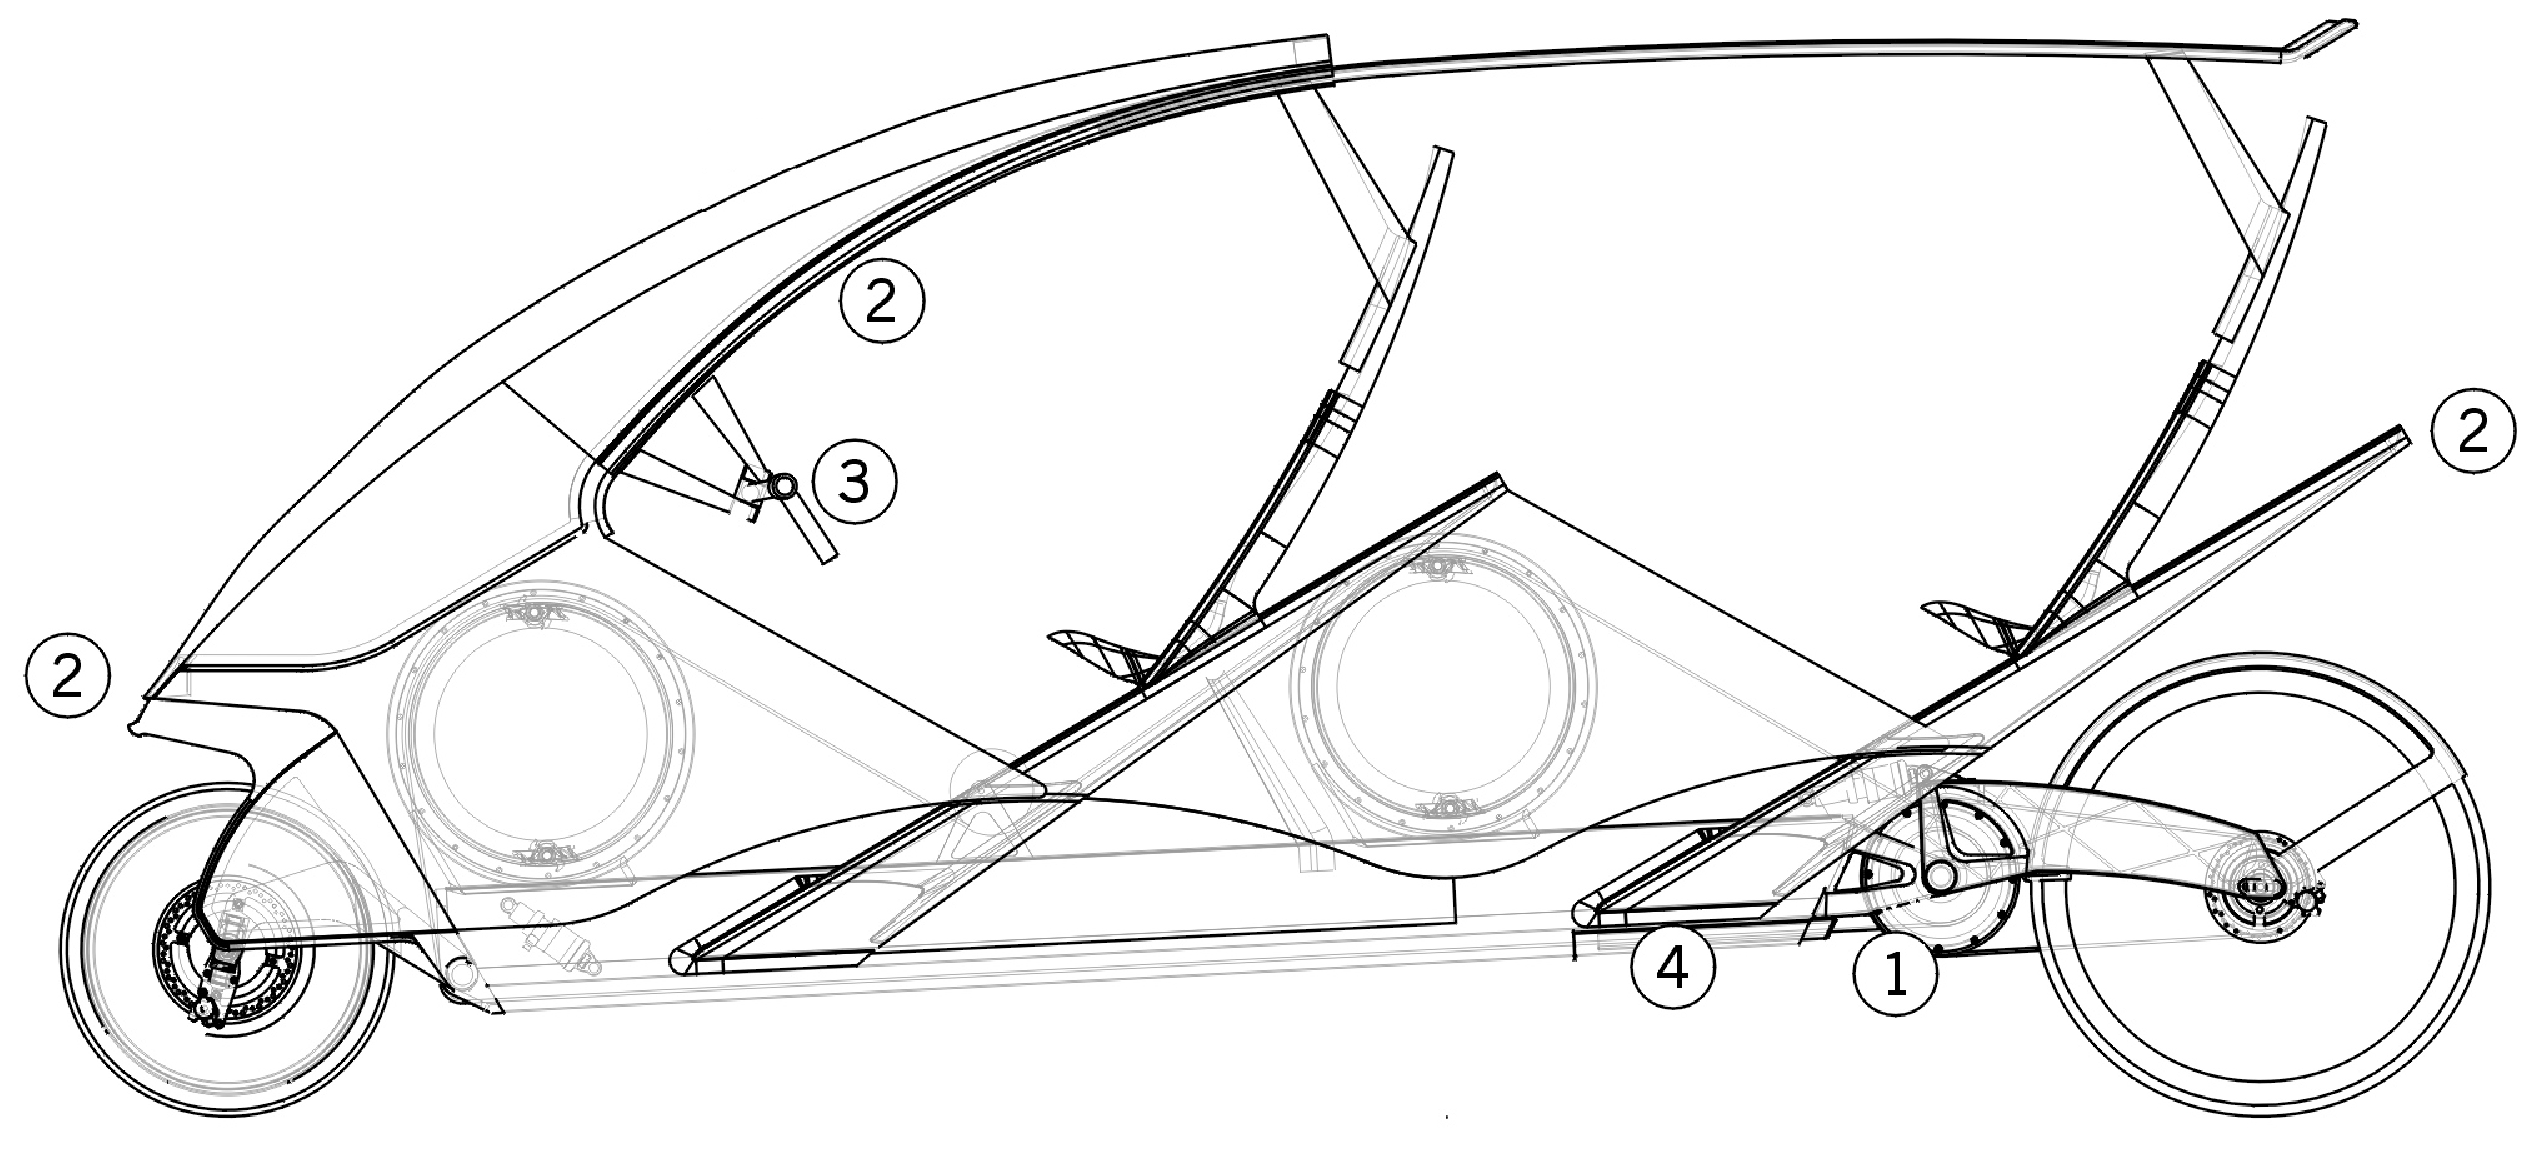
\includegraphics[width=10cm]{laeufer.eps}
      \onlySlide*{1}{Entwicklung eines Mechatronik-Frameworks}%
      \onlySlide*{2}{Platinen samt Mini-Betriebssystem (2)}%
      \onlySlide*{3}{Kommunikation (1-4)}%
      \onlySlide*{4}{Fahrer-Schnittstelle (3)}%
    \end{center}
  \end{slide}
}


% ============================================================


\overlays{4}{%
\begin{slide}{Ziele}
Das erstelle Mechatronik-Framework soll
\begin{itemstep}
  \item sp�ter von den Ingenieuren handhabbar,
  \item durch Industriepartner f�rderbar,
  \item flexibel erweiterbar und
  \item vom Endanwender (L�ufer-Fahrer) akzeptierbar
\end{itemstep}
sein.
\end{slide}
}


% ============================================================


\overlays{4}{%
\begin{slide}{�bersicht �ber das Folgende}
Weg einer Nachricht:
\begin{itemstep}
  \item Benutzer dr�ckt Blinker-Knopf
  \item Weg durch den PDA und die Kommunikation
  \item Umsetzung des Benutzerwunsches auf der Platine
  \item Feststellung eines Fehlers samt Benachrichtigung des Fahrers
\end{itemstep}
\end{slide}
}
